\documentclass[10pt]{article}
\usepackage[T1]{fontenc}
\usepackage{lmodern}
\usepackage[margin=0.7in]{geometry}
\usepackage{amsmath}
\usepackage{microtype}
\usepackage{graphicx}
\usepackage{float}
\usepackage{booktabs}
\usepackage[font=small,labelfont=bf,skip=3pt]{caption}
\captionsetup[figure]{font=footnotesize}
\usepackage[dvipsnames]{xcolor}
\usepackage[colorlinks=true,linkcolor=MidnightBlue,citecolor=MidnightBlue,urlcolor=MidnightBlue]{hyperref}
\usepackage[capitalise]{cleveref}
\setlength{\parskip}{2pt}
\setlength{\parindent}{0pt}
\setlength{\intextsep}{6pt}
\makeatletter
\renewcommand\paragraph{\@startsection{paragraph}{4}{\z@}{1.0ex \@plus .3ex \@minus .2ex}{-1em}{\normalfont\normalsize\bfseries}}
\renewcommand\maketitle{\begin{center}{\large\bfseries\@title\par}\vspace{3pt}\@author\quad\textperiodcentered\quad\@date\end{center}}
\makeatother

\title{Muon with a negative power of the singular values (cross-entropy loss)}
\author{Juntang Wang and V\'ictor Conchello}
\date{November 2026}

\begin{document}
\maketitle
\vspace{-0.8em}

\paragraph{Does a negative power $p$ help under cross-entropy?} At Muon's learning rate (0.01), slightly, but not for the same GPU time. The final validation loss is lowest at $p=-0.3$: 1.3002 against 1.3049 for standard Muon. It rises on both sides, steeply below $p=-0.5$ (\cref{tab:negp}). On three data orders, $p=-0.3$ beats Muon each time, by 0.0047, 0.0015 and 0.0115 (mean 1.3027 against 1.3086); for comparison, Muon's final loss has a standard deviation of 0.0033 over five data orders, so the smallest gain is within noise, but all three have the same sign. At half the rate (0.005), the best power moves towards 0: $p=-0.1$ ends at 1.3016 and $p=0$ at 1.3024, against 1.3077 for standard Muon, while $p=-0.3$ ends at 1.3186; the best run overall is still $p=-0.3$ at rate 0.01. An exact SVD makes each step 9 times slower than Muon's. LC12, a cheap approximation of the $p=-0.3$ update from 12 Newton--Schulz iterates, matches the exact run (mean 1.3020 against 1.3027) at about 1.35 times Muon's step time, but given the GPU time of 10{,}000 Muon steps it ends far behind Muon (1.3337 against 1.3086; \cref{tab:lc}).

\paragraph{What $p$ is.} Our variant takes the SVD $U\,\mathrm{diag}(s)\,V^\top$ of Muon's momentum matrix and updates the weights by $U\,\mathrm{diag}(s^p)\,V^\top$, rescaled to the Frobenius norm of the $p=0$ update. $p=0$ gives every direction the same step: this is Muon with exact orthogonalization; standard Muon approximates it by a Newton--Schulz iteration. $p<0$ gives the largest steps to the directions where the momentum is smallest. For $p<0$, each singular value is divided by the largest one and a ratio below $10^{-6}$ is set to $10^{-6}$ before taking the power.

\paragraph{Runs.} A 14M-parameter GPT on TinyStories, cross-entropy loss, 10{,}000 steps, data order (the shuffling seed) 0 unless stated, on L40S GPUs. Learning rate 0.01 (Muon's best rate with this loss) and half of it. Standard Muon and AdamW (rate 0.002) come from our main Muon-against-AdamW runs: same model, data, steps and GPU type.

\begin{table}[H]
\centering
\small
\caption{Muon with singular values raised to $p$, data order 0. Column 2: the first step at which the training loss reaches 1.81 (the level of our earlier table for $p\ge0$), at rate 0.01. Columns 3--4 at that step: stable rank ($\|W\|_F^2/\sigma_1^2$) and $\sigma_1/\sigma_{\mathrm{median}}$, means over the 36 weight matrices. Column 5: for the rate-0.01 runs, the first step at which the validation loss reaches AdamW's final loss, 1.3391. Columns 6--7: GPU minutes until the validation loss first reaches 1.3391, at either rate: the step there (linear between evaluations) times the method's unrounded time per step (\cref{fig:gputime}); never: not within the 10{,}000 steps. Not run: $p>0$ at rate 0.005, since the minimum at that rate is already bracketed at $p\le0$.}
\label{tab:negp}
\setlength{\tabcolsep}{4pt}
\begin{tabular}{l cccc cc cc}
\toprule
    & step at training & stable & & step at val.\ loss & \multicolumn{2}{c}{GPU min.\ to 1.3391} & \multicolumn{2}{c}{final val.\ loss} \\
run & loss 1.81 & rank & $\sigma_1/\sigma_{\mathrm{median}}$ & 1.3391 & rate 0.01 & rate 0.005 & rate 0.01 & rate 0.005 \\
\midrule
$p=-1$    & 2666 & 2.6  & 37.35 & not reached & never & never & 1.5248 & 1.6232 \\
$p=-0.75$ & 1790 & 3.8  & 21.24 & not reached & never & never & 1.4113 & 1.4524 \\
$p=-0.5$  & 1172 & 8.3  & 9.62  & 9077 & 163.6 & never & 1.3310 & 1.3599 \\
$p=-0.3$  & 959  & 43.2 & 3.80  & 7310 & 131.8 & 145.8 & \textbf{1.3002} & 1.3186 \\
$p=-0.1$  & 817  & 98.2 & 2.44  & 7549 & 136.1 & 131.6 & 1.3035 & \textbf{1.3016} \\
$p=0$     & 847  & 87.7 & 2.65  & 7521 & 135.6 & 132.9 & 1.3046 & 1.3024 \\
$p=0.25$  & 965  & 64.1 & 3.38  & 8463 & 152.5 & not run & 1.3250 & not run \\
$p=0.5$   & 1132 & 39.1 & 5.34  & 9348 & 168.5 & not run & 1.3351 & not run \\
$p=0.75$  & 1432 & 32.9 & 9.06  & not reached & never & not run & 1.3601 & not run \\
\midrule
Muon (Newton--Schulz) & 868 & 86.5 & 2.68 & 7474 & \textbf{14.6} & \textbf{15.1} & 1.3049 & 1.3077 \\
LC12 (\cref{tab:lc}) & 938 & -- & -- & 7366 & 19.5 & -- & 1.3006 & -- \\
AdamW (rate 0.002) & 1438 & 32.9 & 7.95 & 10000 & 17.9 & -- & 1.3391 & -- \\
\bottomrule
\end{tabular}
\end{table}

\begin{figure}[H]
\centering
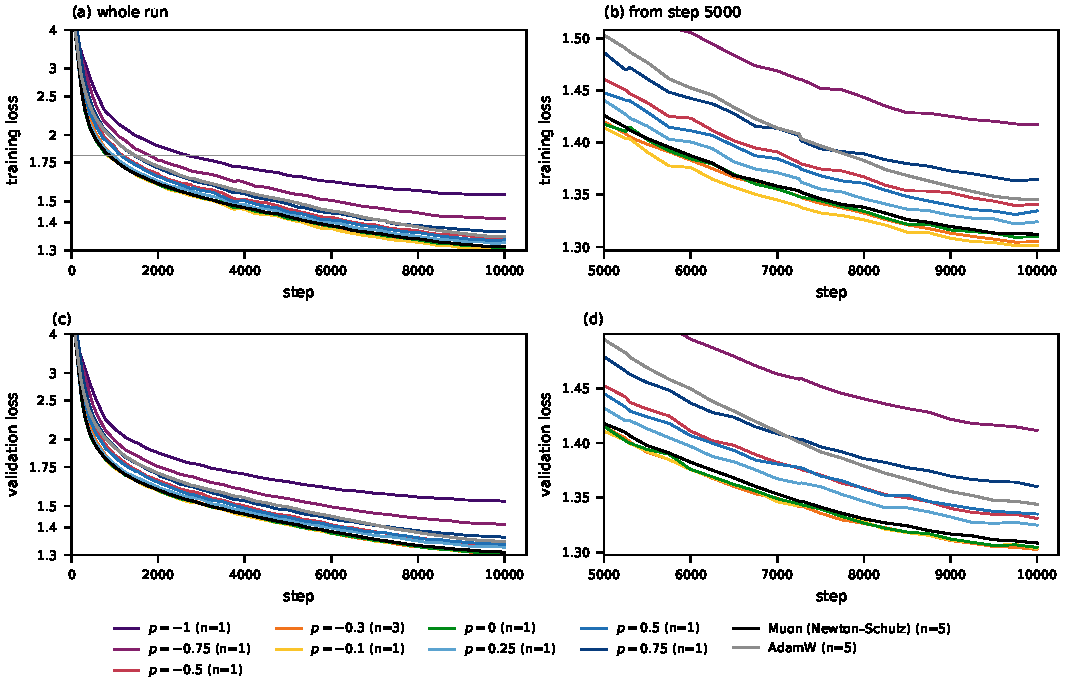
\includegraphics[width=\linewidth]{ts10m/dose_loss_ce.pdf}
\caption{Training (top) and validation (bottom) loss at rate 0.01, data order 0, one colour per $p$ (yellow to dark purple: negative; blue: positive; black: $p=0$). Left: the whole run, loss axis logarithmic in (loss $-$ 1); the horizontal line is the loss 1.81 of \cref{tab:negp}. Right: from step 5000 on, linear axis capped at AdamW's loss at step 5000; curves above it are cut off.}
\label{fig:loss}
\end{figure}

\paragraph{Paths.} We measure how far each run is from standard Muon on the same data order by the mean Jensen--Shannon divergence (JS, in bits) of their next-token predictions on held-out text, as in Fig.~1 of our checkpoint report. AdamW on the same data order is the reference: like the $p$ runs, it sees the same batches as Muon. From $p=-0.3$ to $p=0.25$, a run is closer to Muon than AdamW is, at equal step and at equal training loss (\cref{fig:paths}; at loss 1.81, $p=-0.3$ is at 0.079 bits and AdamW at 0.122). So $p=-0.3$ changes the path less than switching to AdamW does, yet it lowers the final loss on all three data orders. At equal loss, $p=-0.5$, $p=0.5$ and $p=0.75$ are about as far from Muon as AdamW is, and $p\le-0.75$ farther.

\begin{figure}[H]
\centering
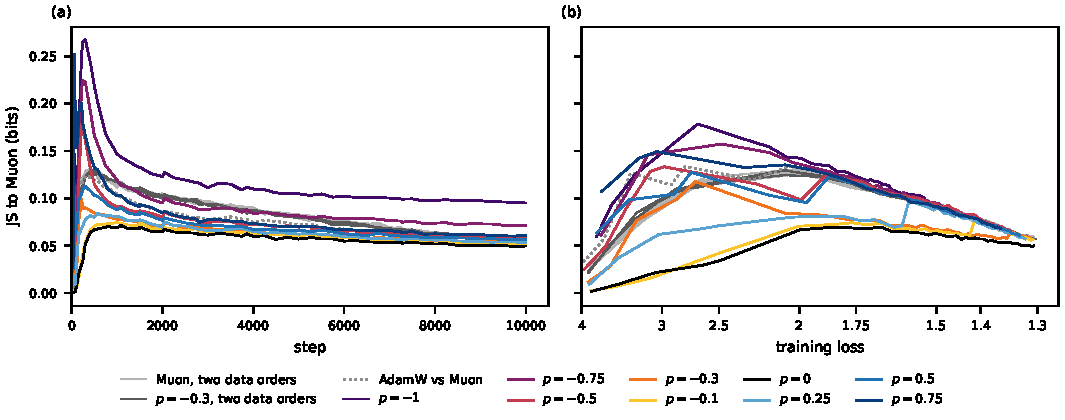
\includegraphics[width=\linewidth]{ts10m/dose_paths_ce.pdf}
\caption{JS between each run (data order 0, rate 0.01) and standard Muon on the same data order. (a) At equal step. (b) At equal training loss: each checkpoint (one every 250 steps) is compared with two Muon checkpoints, those just before and after the step where Muon's smoothed training loss equals the run's, and the smaller JS is kept. Dotted: AdamW against Muon. Grey: two data orders of Muon (light) or of $p=-0.3$ (dark), which share no batches. Runs on one data order agree much more at the same step, having just seen the same batches; so a curve in (b) jumps up when its matched Muon checkpoint is no longer at its own step ($p=0.25$ at loss 1.6).}
\label{fig:paths}
\end{figure}

\paragraph{A cheaper update (LC).} LC$k$ (linear combination) approximates the $p=-0.3$ update by a weighted sum of the first $k$ Newton--Schulz iterates (3 matrix products each), with weights fitted for $p=-0.3$; standard Muon uses 5 iterates. We ran LC with 5, 6, 8 and 12 iterates on three data orders (\cref{tab:lc}, \cref{fig:lc}). LC12 matches the exact update on average (1.3020 against 1.3027) at about 1.35 times Muon's step time, and LC8 comes close (1.3037). Measured in GPU time, none beats Muon (\cref{tab:lc,fig:gputime}): Muon reaches its own final loss after about 19 minutes, LC5 to LC12 after 19--25 minutes when they reach it at all. Given exactly Muon's GPU time, LC12 ends at 1.3337, far behind Muon's 1.3086: shrinking the schedule costs more than the better update gains. In our earlier runs with the MSE loss, another approximation (two-track Newton--Schulz, 12 steps) also matched the exact update (0.5628 against 0.5626), but it costs 47 matrix products to LC12's 36, so we skipped it here.

\begin{table}[H]
\centering
\small
\caption{Cheaper updates at $p=-0.3$, rate 0.01, data orders 0--2. ms per step: from one timing job on one L40S, each method run as two copies side by side. GPU minutes = steps $\times$ ms per step. Error: relative distance $\|Z-E\|_F/\|E\|_F$ between the update $Z$ and the exact one $E$, median over the 36 matrices and the logged steps, up to nine (the exact row: float32 against float64). Columns 9--11: GPU time until the validation loss reaches standard Muon's final one on the same data order. Last column: GPU time until it reaches 1.3391 (AdamW's final loss on d0, the same level for every data order), mean over d0--d2; \cref{tab:negp} gives d0 alone. LC12 at equal GPU time: LC12 with its whole schedule (warmup and decay) shrunk to 7391 steps, the GPU time of 10{,}000 Muon steps.}
\label{tab:lc}
\setlength{\tabcolsep}{2.8pt}
\begin{tabular}{l ccc cccc ccc c}
\toprule
 & matrix & ms per & & \multicolumn{4}{c}{final val.\ loss} & \multicolumn{3}{c}{GPU minutes to Muon's loss} & GPU min.\ to \\
method & products & step & error & d0 & d1 & d2 & mean & d0 & d1 & d2 & 1.3391 \\
\midrule
exact SVD & -- & 1081 & 0.000 & 1.3002 & 1.3055 & 1.3023 & 1.3027 & 166 & 175 & 158 & 132.8 \\
LC12 & 36 & 159 & 0.044 & 1.3006 & 1.3032 & 1.3021 & \textbf{1.3020} & 24.3 & 24.8 & 23.1 & 19.4 \\
LC8  & 24 & 142 & 0.409 & 1.3024 & 1.3021 & 1.3067 & 1.3037 & 23.3 & 22.5 & 21.8 & 17.6 \\
LC6  & 18 & 126 & 0.570 & 1.3080 & 1.3066 & 1.3073 & 1.3073 & never & 20.9 & 19.3 & 15.9 \\
LC5  & 15 & 123 & 0.696 & 1.3108 & 1.3092 & 1.3126 & 1.3109 & never & never & 20.1 & 15.8 \\
LC12, equal GPU time & 36 & 159 & 0.044 & 1.3351 & 1.3331 & 1.3330 & 1.3337 & never & never & never & 18.5 \\
\midrule
Muon (Newton--Schulz) & 15 & 117 & -- & 1.3049 & 1.3070 & 1.3138 & 1.3086 & \textbf{19.5} & \textbf{19.5} & \textbf{18.9} & \textbf{14.8} \\
\bottomrule
\end{tabular}
\end{table}

\begin{figure}[H]
\centering
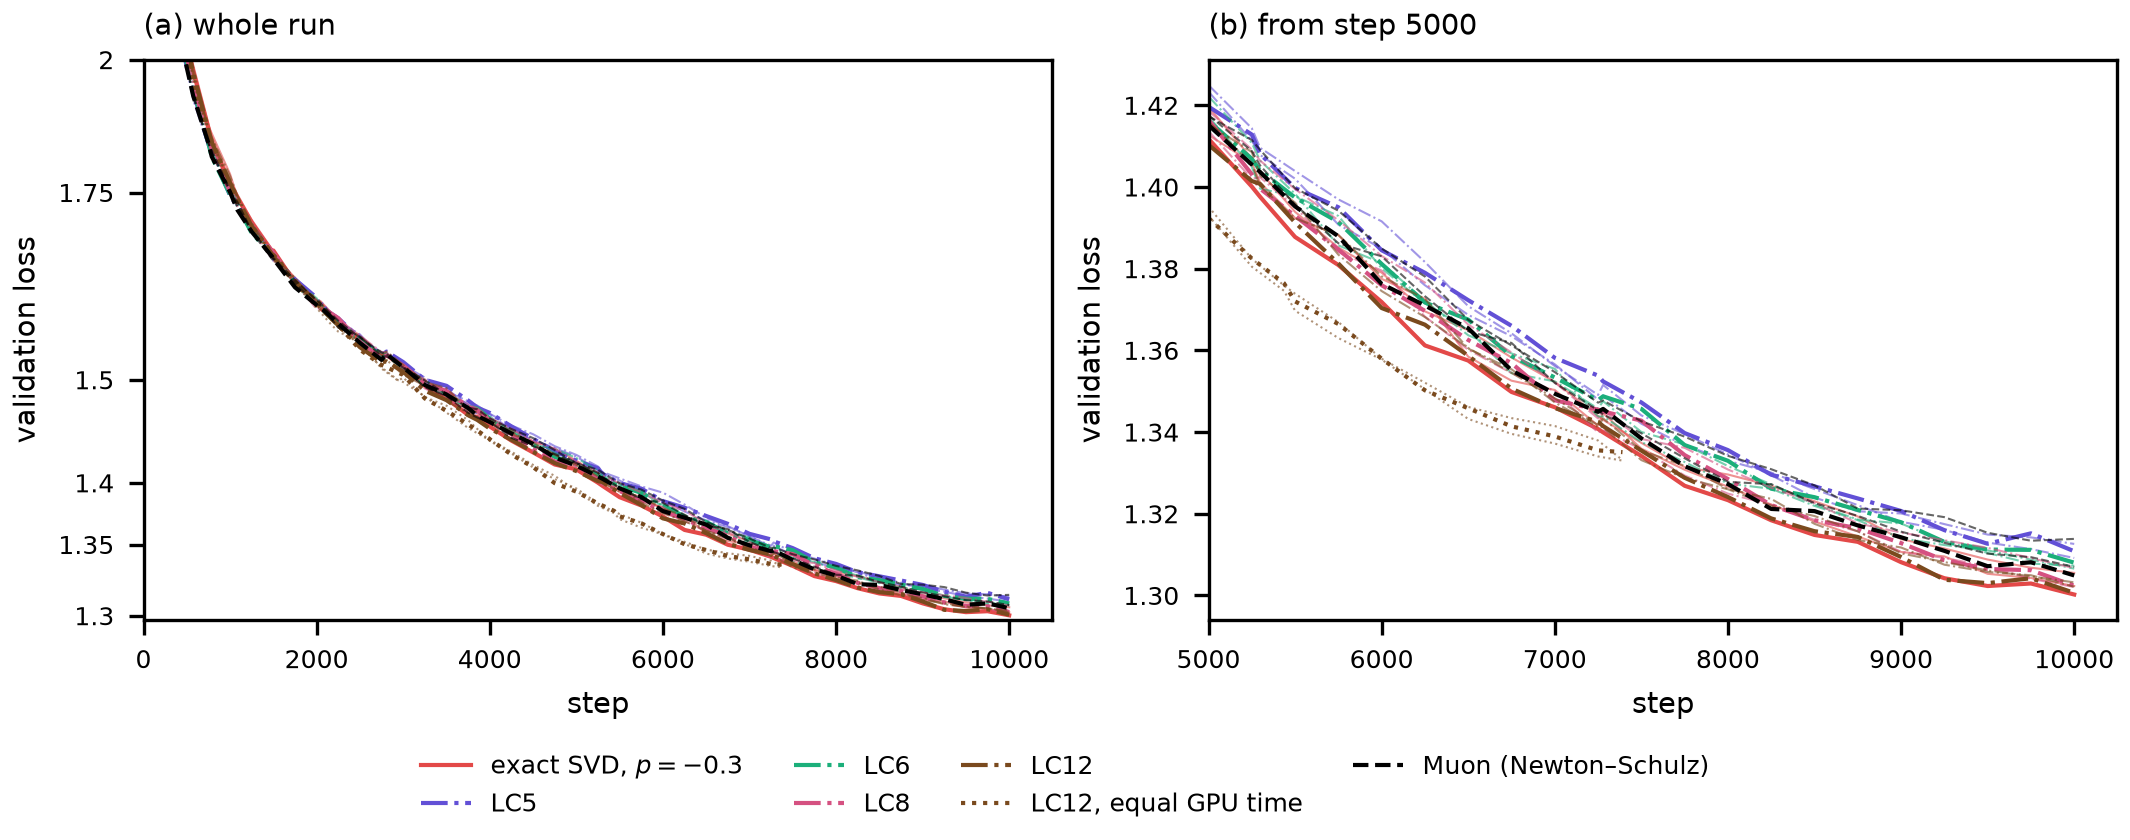
\includegraphics[width=\linewidth]{ts10m/two_track_val_ce.png}
\caption{Validation loss of the methods of \cref{tab:lc}; data order 0 thick, 1 and 2 thin. (a) The whole run, loss axis logarithmic in (loss $-$ 1). (b) From step 5000 on. LC12 at equal GPU time ends at step 7391; its learning rate decays earlier, so it is lower mid-run but ends higher.}
\label{fig:lc}
\end{figure}

\begin{figure}[H]
\centering
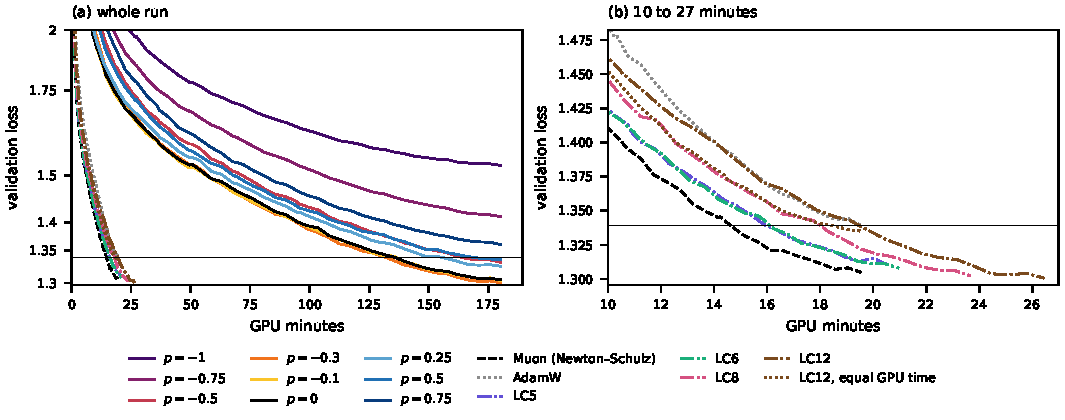
\includegraphics[width=\linewidth]{ts10m/gpu_time_val_ce.pdf}
\caption{Validation loss against GPU time, rate 0.01 (AdamW 0.002), data order 0. GPU time = step $\times$ the method's time per step, measured in short timing jobs on one L40S (400 steps, without the Hessian and other measurements made during the long runs; the time per step of one run while a second identical run shares the GPU): Muon 117, LC5/6/8/12 123/126/142/159 and exact SVD 1081 ms per step (timed at $p=-0.3$, used for every $p$). AdamW: 107 ms per step, timed the same way in a second job (an earlier pilot gave 108 ms). The logged wall-clock is not used: the long runs shared GPUs, and some of them measured the Hessian. Horizontal line: AdamW's final loss, 1.3391, the level of the columns ``GPU min.\ to 1.3391'' of \cref{tab:negp,tab:lc}. (a) The whole run, loss axis logarithmic in (loss $-$ 1). (b) 10 to 27 minutes, linear axis capped at AdamW's loss at 10 minutes; the exact-SVD runs are still above it.}
\label{fig:gputime}
\end{figure}

% Written by code/scripts/lc5m_section.py (scripts/lc5m_section.sh); edits here are overwritten.
\clearpage
\paragraph{LC5m: LC5 with a Muon floor (in progress).} LC5m is LC5 (\cref{tab:lc}) with a hard constraint: every singular value of its update lies between Muon's value and the exact $s^{-0.3}$.

\begin{table}[H]
\centering
\small
\caption{LC5m, one row per data order. GPU minutes until the validation loss first reaches 1.3391, as in \cref{tab:negp,tab:lc}; ms per step: Muon 117, LC5 123, exact 1081, AdamW 107, LC5m 123 (timed as LC5 until its own timing pilot has run). Exact: exact SVD, $p=-0.3$. running: not finished; --: not run. Mean: over the orders where LC5m has finished (none yet).}
\label{tab:lc5m}
\setlength{\tabcolsep}{3.5pt}
\begin{tabular}{l ccccc ccccc}
\toprule
 & \multicolumn{5}{c}{final val.\ loss} & \multicolumn{5}{c}{GPU min.\ to 1.3391} \\
\cmidrule(lr){2-6}\cmidrule(lr){7-11}
order & LC5m & Muon & LC5 & exact & AdamW & LC5m & Muon & LC5 & exact & AdamW \\
\midrule
d0 & running & 1.3049 & 1.3108 & 1.3002 & 1.3391 & running & 14.6 & 16.0 & 131.8 & 17.9 \\
d1 & running & 1.3070 & 1.3092 & 1.3055 & 1.3462 & running & 14.7 & 15.7 & 133.9 & never \\
d2 & running & 1.3138 & 1.3126 & 1.3023 & 1.3446 & running & 15.1 & 15.9 & 132.6 & never \\
d3 & running & 1.3084 & -- & -- & 1.3496 & running & 14.9 & -- & -- & never \\
d4 & running & 1.3090 & -- & -- & 1.3403 & running & 15.1 & -- & -- & never \\
\midrule
mean & -- & -- & -- & -- & -- & -- & -- & -- & -- & -- \\
\bottomrule
\end{tabular}
\end{table}

\begin{figure}[H]
\centering
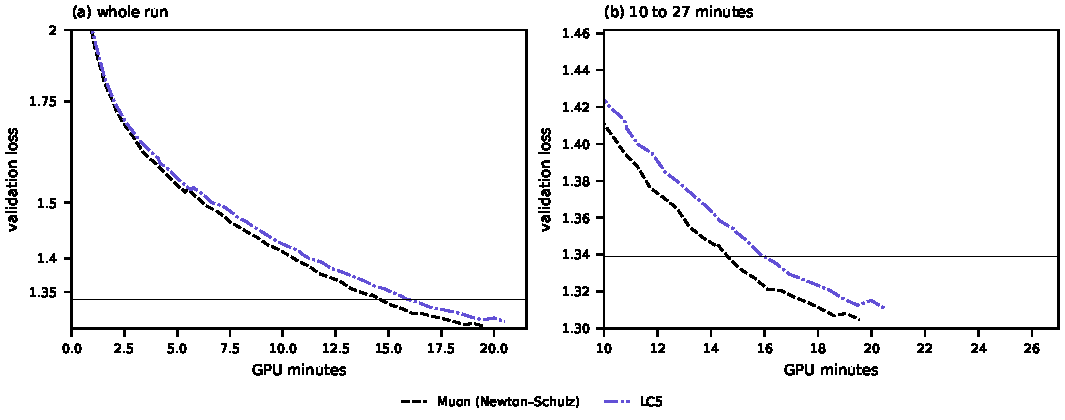
\includegraphics[width=\linewidth]{ts10m/lc5m_gpu_time_ce.pdf}
\caption{As \cref{fig:gputime}, for LC5m, LC5 and Muon on data order 0 (no LC5m run has finished yet).}
\label{fig:lc5m}
\end{figure}
  % written by code/scripts/lc5m_section.sh

\end{document}
